% GNUPLOT: LaTeX picture with Postscript
\begingroup
  \makeatletter
  \providecommand\color[2][]{%
    \GenericError{(gnuplot) \space\space\space\@spaces}{%
      Package color not loaded in conjunction with
      terminal option `colourtext'%
    }{See the gnuplot documentation for explanation.%
    }{Either use 'blacktext' in gnuplot or load the package
      color.sty in LaTeX.}%
    \renewcommand\color[2][]{}%
  }%
  \providecommand\includegraphics[2][]{%
    \GenericError{(gnuplot) \space\space\space\@spaces}{%
      Package graphicx or graphics not loaded%
    }{See the gnuplot documentation for explanation.%
    }{The gnuplot epslatex terminal needs graphicx.sty or graphics.sty.}%
    \renewcommand\includegraphics[2][]{}%
  }%
  \providecommand\rotatebox[2]{#2}%
  \@ifundefined{ifGPcolor}{%
    \newif\ifGPcolor
    \GPcolorfalse
  }{}%
  \@ifundefined{ifGPblacktext}{%
    \newif\ifGPblacktext
    \GPblacktexttrue
  }{}%
  % define a \g@addto@macro without @ in the name:
  \let\gplgaddtomacro\g@addto@macro
  % define empty templates for all commands taking text:
  \gdef\gplbacktext{}%
  \gdef\gplfronttext{}%
  \makeatother
  \ifGPblacktext
    % no textcolor at all
    \def\colorrgb#1{}%
    \def\colorgray#1{}%
  \else
    % gray or color?
    \ifGPcolor
      \def\colorrgb#1{\color[rgb]{#1}}%
      \def\colorgray#1{\color[gray]{#1}}%
      \expandafter\def\csname LTw\endcsname{\color{white}}%
      \expandafter\def\csname LTb\endcsname{\color{black}}%
      \expandafter\def\csname LTa\endcsname{\color{black}}%
      \expandafter\def\csname LT0\endcsname{\color[rgb]{1,0,0}}%
      \expandafter\def\csname LT1\endcsname{\color[rgb]{0,1,0}}%
      \expandafter\def\csname LT2\endcsname{\color[rgb]{0,0,1}}%
      \expandafter\def\csname LT3\endcsname{\color[rgb]{1,0,1}}%
      \expandafter\def\csname LT4\endcsname{\color[rgb]{0,1,1}}%
      \expandafter\def\csname LT5\endcsname{\color[rgb]{1,1,0}}%
      \expandafter\def\csname LT6\endcsname{\color[rgb]{0,0,0}}%
      \expandafter\def\csname LT7\endcsname{\color[rgb]{1,0.3,0}}%
      \expandafter\def\csname LT8\endcsname{\color[rgb]{0.5,0.5,0.5}}%
    \else
      % gray
      \def\colorrgb#1{\color{black}}%
      \def\colorgray#1{\color[gray]{#1}}%
      \expandafter\def\csname LTw\endcsname{\color{white}}%
      \expandafter\def\csname LTb\endcsname{\color{black}}%
      \expandafter\def\csname LTa\endcsname{\color{black}}%
      \expandafter\def\csname LT0\endcsname{\color{black}}%
      \expandafter\def\csname LT1\endcsname{\color{black}}%
      \expandafter\def\csname LT2\endcsname{\color{black}}%
      \expandafter\def\csname LT3\endcsname{\color{black}}%
      \expandafter\def\csname LT4\endcsname{\color{black}}%
      \expandafter\def\csname LT5\endcsname{\color{black}}%
      \expandafter\def\csname LT6\endcsname{\color{black}}%
      \expandafter\def\csname LT7\endcsname{\color{black}}%
      \expandafter\def\csname LT8\endcsname{\color{black}}%
    \fi
  \fi
    \setlength{\unitlength}{0.0500bp}%
    \ifx\gptboxheight\undefined%
      \newlength{\gptboxheight}%
      \newlength{\gptboxwidth}%
      \newsavebox{\gptboxtext}%
    \fi%
    \setlength{\fboxrule}{0.5pt}%
    \setlength{\fboxsep}{1pt}%
\begin{picture}(5668.00,3968.00)%
    \gplgaddtomacro\gplbacktext{%
      \csname LTb\endcsname%%
      \put(434,2918){\makebox(0,0)[r]{\strut{}$0$}}%
      \csname LTb\endcsname%%
      \put(434,3221){\makebox(0,0)[r]{\strut{}$0.6$}}%
      \csname LTb\endcsname%%
      \put(434,3523){\makebox(0,0)[r]{\strut{}$1.2$}}%
      \csname LTb\endcsname%%
      \put(434,3826){\makebox(0,0)[r]{\strut{}$1.8$}}%
      \csname LTb\endcsname%%
      \put(566,2597){\makebox(0,0){\strut{}}}%
      \csname LTb\endcsname%%
      \put(967,2597){\makebox(0,0){\strut{}}}%
      \csname LTb\endcsname%%
      \put(1369,2597){\makebox(0,0){\strut{}}}%
      \csname LTb\endcsname%%
      \put(1770,2597){\makebox(0,0){\strut{}}}%
      \csname LTb\endcsname%%
      \put(2172,2597){\makebox(0,0){\strut{}}}%
      \csname LTb\endcsname%%
      \put(2573,2597){\makebox(0,0){\strut{}}}%
      \csname LTb\endcsname%%
      \put(2975,2597){\makebox(0,0){\strut{}}}%
      \csname LTb\endcsname%%
      \put(3376,2597){\makebox(0,0){\strut{}}}%
      \csname LTb\endcsname%%
      \put(3777,2597){\makebox(0,0){\strut{}}}%
      \csname LTb\endcsname%%
      \put(4179,2597){\makebox(0,0){\strut{}}}%
      \csname LTb\endcsname%%
      \put(4580,2597){\makebox(0,0){\strut{}}}%
      \csname LTb\endcsname%%
      \put(4982,2597){\makebox(0,0){\strut{}}}%
      \csname LTb\endcsname%%
      \put(5383,2597){\makebox(0,0){\strut{}}}%
    }%
    \gplgaddtomacro\gplfronttext{%
      \csname LTb\endcsname%%
      \put(-171,3372){\rotatebox{-270}{\makebox(0,0){\strut{}$V_{out}$ $[V]$}}}%
      \put(2974,2531){\makebox(0,0){\strut{}}}%
    }%
    \gplgaddtomacro\gplbacktext{%
      \csname LTb\endcsname%%
      \put(434,1807){\makebox(0,0)[r]{\strut{}$0$}}%
      \csname LTb\endcsname%%
      \put(434,2110){\makebox(0,0)[r]{\strut{}$0.6$}}%
      \csname LTb\endcsname%%
      \put(434,2412){\makebox(0,0)[r]{\strut{}$1.2$}}%
      \csname LTb\endcsname%%
      \put(434,2715){\makebox(0,0)[r]{\strut{}$1.8$}}%
      \csname LTb\endcsname%%
      \put(566,1486){\makebox(0,0){\strut{}}}%
      \csname LTb\endcsname%%
      \put(967,1486){\makebox(0,0){\strut{}}}%
      \csname LTb\endcsname%%
      \put(1369,1486){\makebox(0,0){\strut{}}}%
      \csname LTb\endcsname%%
      \put(1770,1486){\makebox(0,0){\strut{}}}%
      \csname LTb\endcsname%%
      \put(2172,1486){\makebox(0,0){\strut{}}}%
      \csname LTb\endcsname%%
      \put(2573,1486){\makebox(0,0){\strut{}}}%
      \csname LTb\endcsname%%
      \put(2975,1486){\makebox(0,0){\strut{}}}%
      \csname LTb\endcsname%%
      \put(3376,1486){\makebox(0,0){\strut{}}}%
      \csname LTb\endcsname%%
      \put(3777,1486){\makebox(0,0){\strut{}}}%
      \csname LTb\endcsname%%
      \put(4179,1486){\makebox(0,0){\strut{}}}%
      \csname LTb\endcsname%%
      \put(4580,1486){\makebox(0,0){\strut{}}}%
      \csname LTb\endcsname%%
      \put(4982,1486){\makebox(0,0){\strut{}}}%
      \csname LTb\endcsname%%
      \put(5383,1486){\makebox(0,0){\strut{}}}%
    }%
    \gplgaddtomacro\gplfronttext{%
      \csname LTb\endcsname%%
      \put(-171,2261){\rotatebox{-270}{\makebox(0,0){\strut{}$V_{in,1}$ $[V]$}}}%
      \put(2974,1420){\makebox(0,0){\strut{}}}%
    }%
    \gplgaddtomacro\gplbacktext{%
      \csname LTb\endcsname%%
      \put(434,696){\makebox(0,0)[r]{\strut{}$0$}}%
      \csname LTb\endcsname%%
      \put(434,999){\makebox(0,0)[r]{\strut{}$0.6$}}%
      \csname LTb\endcsname%%
      \put(434,1301){\makebox(0,0)[r]{\strut{}$1.2$}}%
      \csname LTb\endcsname%%
      \put(434,1604){\makebox(0,0)[r]{\strut{}$1.8$}}%
      \csname LTb\endcsname%%
      \put(566,375){\makebox(0,0){\strut{}0}}%
      \csname LTb\endcsname%%
      \put(967,375){\makebox(0,0){\strut{}1.5}}%
      \csname LTb\endcsname%%
      \put(1369,375){\makebox(0,0){\strut{}3}}%
      \csname LTb\endcsname%%
      \put(1770,375){\makebox(0,0){\strut{}4.5}}%
      \csname LTb\endcsname%%
      \put(2172,375){\makebox(0,0){\strut{}6}}%
      \csname LTb\endcsname%%
      \put(2573,375){\makebox(0,0){\strut{}7.5}}%
      \csname LTb\endcsname%%
      \put(2975,375){\makebox(0,0){\strut{}9}}%
      \csname LTb\endcsname%%
      \put(3376,375){\makebox(0,0){\strut{}10.5}}%
      \csname LTb\endcsname%%
      \put(3777,375){\makebox(0,0){\strut{}12}}%
      \csname LTb\endcsname%%
      \put(4179,375){\makebox(0,0){\strut{}13.5}}%
      \csname LTb\endcsname%%
      \put(4580,375){\makebox(0,0){\strut{}15}}%
      \csname LTb\endcsname%%
      \put(4982,375){\makebox(0,0){\strut{}16.5}}%
      \csname LTb\endcsname%%
      \put(5383,375){\makebox(0,0){\strut{}18}}%
    }%
    \gplgaddtomacro\gplfronttext{%
      \csname LTb\endcsname%%
      \put(-171,1150){\rotatebox{-270}{\makebox(0,0){\strut{}$V_{in,2}$ $[V]$}}}%
      \put(2974,45){\makebox(0,0){\strut{}tempo $[ns]$}}%
    }%
    \gplbacktext
    \put(0,0){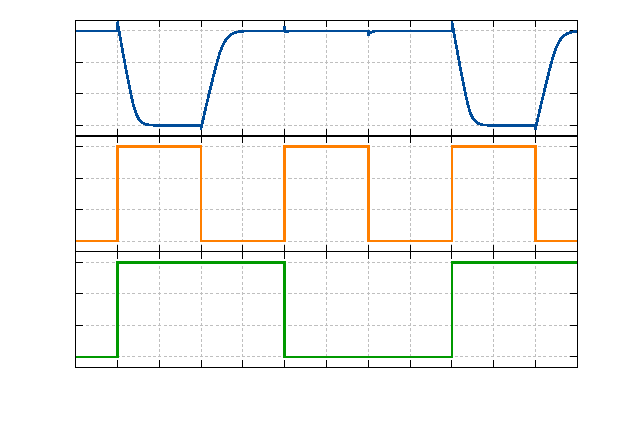
\includegraphics[width={283.40bp},height={198.40bp}]{Immagini/nand-dinamica}}%
    \gplfronttext
  \end{picture}%
\endgroup

